\documentclass[../thesis.tex]{subfiles}

\begin{document}


% Deep IRL in off-road environment

Most of the robotics problems can be formulated in optimization problems. For the motion planning problems, the objectives are defined as finding a sequence of control actions that minimize the accumulated costs toward the goal state. Reinforcement learning on the other hand tries to learn a optimal policy that maximizes the expected accumulated rewards in the environment. 

It is worth mentioning that unlike the urban environment where rewards are well defined in a rule-based structure, finding a cost function for off-road navigation can be nontrivial and often requires lot of handy tuning. 
The problem thus naturally fits with inverse reinforcement learning, in which the principle goal is to infer the \textit{cost} function of a policy given the pairs of observations and the its corresponding actions.

Here, followed by the previous success \cite{wulfmeier2015maximum,wulfmeier2016watch} of using deep neural net to approximate the cost function, we implemented a similar algorithm for off-road application. 

\section{Proposed Methods}

\subsection{Construct Feature Maps}

\begin{figure}[t]
	\begin{center}
		\centerline{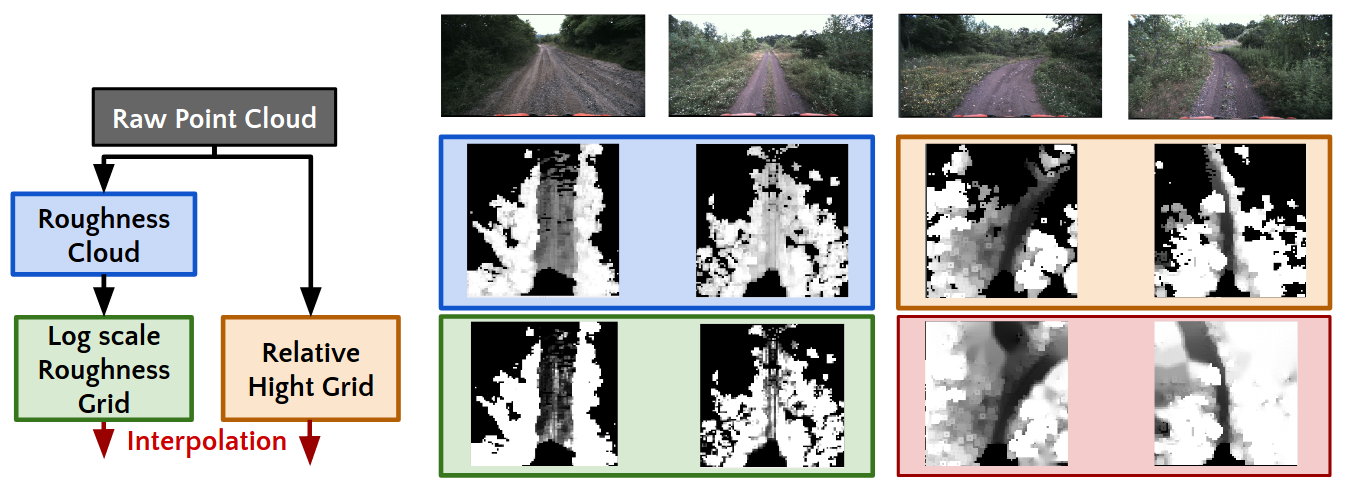
\includegraphics[width=\columnwidth]{./DIRL/fig/lidar_feature_map.png}}
		\caption{The extracted feature maps from LiDAR. The flow chart is shown on the left of the figure, while examples of the actual collected data on filed are shown on the right of the figure.}
		\label{fig:lidar_feature_map}
	\end{center}
\end{figure} 

Following Chapter \ref{chap:rrtplanner}, 
% Section \ref{sec:rrt-experiments}, 
we use Yamaha Viking VI side-by-side ATV as our main testing platform.
Under the variety of available on-board sensors, we pick LiDAR as our primary input since it is more reliable and informative features such as terrain roughness can be inferred straight-forwardly.

We first divide the incoming point cloud into patch structures. For each patch, a normal plane is calculated using standard least square regression. Once the normal plane parameters is calculated, we define the \textit{roughness index} as the average plane variance with respect to each . 
However, the naive roughness index is sensitive to hypaerparameter such as patch size and rescaling factors. In the off-road environment where the terrain can vary a lot, this approach can fail to extracted reasonable feature when trail becomes narrow, as shown in the second column of Fig. \ref{fig:lidar_feature_map}. 
To alleviate this issue, we replace the original roughness index with log-scale value. The log scaling help amplify the slight difference among traversible terrains, and flatten the non-traversible terrain such as bush or trees. 
The second feature map we use is the relative hight with respect to the vehicle local frame. 

For off-road environment, it is common that scenes are blocked by un-structured obstacles, resulting in the empty region that degrades the performance of the learn cost map. 
To alleviate this issue, we apply a standard image in-painting technique \cite{telea2004image} 
that effectively help infer the the invisible region given the geometric shape of the visible trails. 
The feature maps before and after interpolation are shown in the orange and red area in Fig. \ref{fig:lidar_feature_map}, respectively.



% Learning from Failure + Gibbs distribution
\subsection{Learning from Failure for DIRL}

%%% Challenge %%% 

One of the challenges rises with DIRL is the spatially sparse gradient feedback. As mentioned clearly in \cite{wulfmeier2016incorporating}, the loss signals during DIRL training focus more on the region around the demonstration trajectories. 
% Since the gradient comes from the difference between two demonstration and maximum entropy distribution, the neural network will inherently focus more around the sample data. 
The problem can be alleviated by pre-training the network under standard image segmentation framework, which provide a pixel-wise feedback for error terms. Here, we propose an alternative approach that re-formulated the some problem with \textit{negative} demonstrations.

Following the same convention in Section \ref{sec:dirl}, we now denote the positive and negative demonstration as $D_{pos}$ and $D_{neg}$, respectively. The log likelihood (Eq. \ref{equ:irl_obj}) can be reformulated as:

\begin{align}
L(\theta) &= \log P(D_{pos}, D_{neg},\theta|r) \\
&= \log P(D_{pos}|r) + \log P(D_{neg}|r^{-1}) + \log P(\theta)
\end{align}

With the L2-regularization, the new gradient descent becomes:

\begin{align}
\frac{\partial L}{\partial \theta} &= \left( \mu_{D_{pos}} - \mathbb{E}_{r}[\mu] \right) \frac{\partial r}{\partial \theta} + \left( \mu_{D_{neg}} - \mathbb{E}_{r^{-1}}[\mu] \right) \frac{\partial r^{-1}}{\partial r} \frac{\partial r}{\partial \theta} + \frac{\lambda}{2} \| \theta \|^2 \\
&= \left( \mu_{D_{pos}} - \mathbb{E}_{r}[\mu] + \mathbb{E}_{r^{-1}}[\mu] - \mu_{D_{neg}} \right) \cdot \frac{\partial r}{\partial \theta} + \frac{\lambda}{2} \| \theta \|^2
\end{align}

where $r^{-1} = constant - r $ stands for \textit{inverted} reward map. 

By jointly optimizing with the negative demonstrations, we can increase the gradient signals for non-traversible 


\section{Experiments Results}


\begin{figure}[t]
	\begin{center}
		\centerline{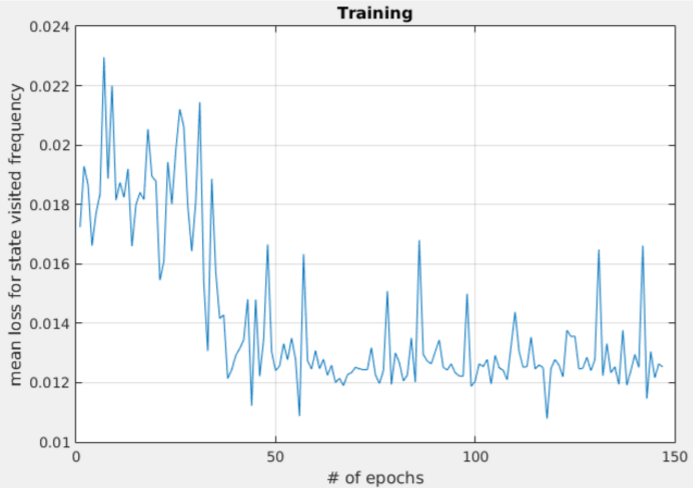
\includegraphics[width=0.3\columnwidth]{./DIRL/fig/dirl_training_curve.png}}
		\caption{Training curve of DIRL in Gascola dataset.}
		\label{fig:dirl_learning_curve}
	\end{center}
\end{figure} 

\begin{figure}[t]
	\begin{center}
		\centerline{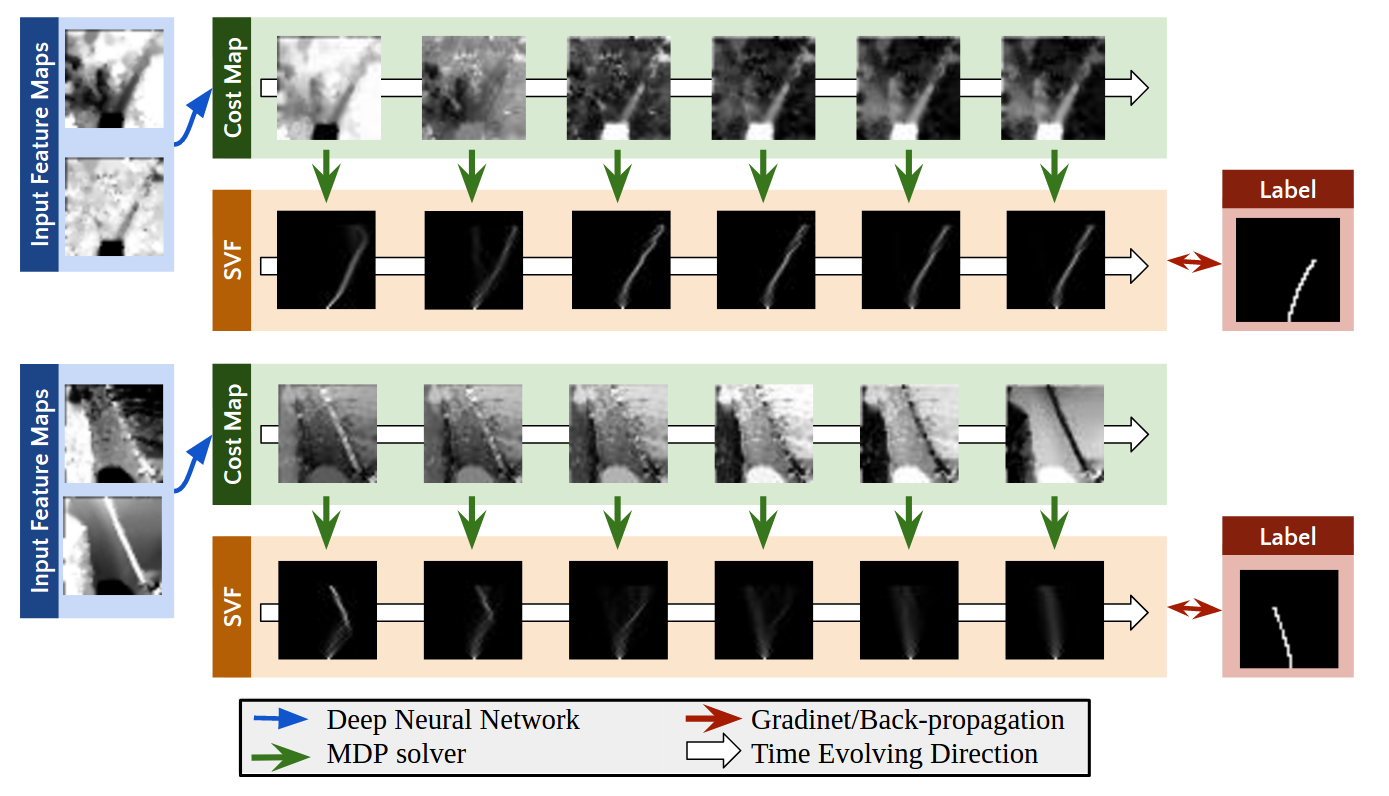
\includegraphics[width=0.8\columnwidth]{./DIRL/fig/inter_cost_map.png}}
		\caption{Samples of intermediate cost maps during training.}
		\label{fig:inter_cost_map}
	\end{center}
\end{figure} 


The dataset contains total 150 human demonstrations covering an off-road testing field at Gascola, PA. Each sample covers the $20m \times 20m$ region in front of the ATV. Since the Gascola dataset is relatively small, we use a shallow multilayer perception as the cost function. 
The training curve is summarized in Fig. \ref{fig:dirl_learning_curve}. 
Two testing examples of the intermediate cost maps during training are visualized in Fig. \ref{fig:inter_cost_map}. 


% \subsection{Intersection Handling}

\end{document}